\documentclass[11pt]{scrartcl}
\usepackage[utf8]{inputenc}
\usepackage[croatian]{babel}
\usepackage{datetime}
\newdate{date}{08}{06}{2024}
\date{\displaydate{date}}
\usepackage[a4paper,margin=1in]{geometry}
\usepackage{amsfonts}
\usepackage{amsmath}
\usepackage{amssymb}
\usepackage{amsthm}
\usepackage{csquotes}
\usepackage{tcolorbox}
\usepackage{tikz}
\usepackage{arydshln}
\pagenumbering{gobble}
\usepackage{float}
\usepackage{xcolor}
%\usepackage[dvipsnames]{xcolor}
%\usepackage{mathptmx} %times new roman?
\usepackage{breqn}
\usepackage[T1]{fontenc}
\usepackage{thmtools}
\usepackage{multirow}
\usepackage[unicode]{hyperref}

\usepackage{booktabs}
\usepackage{listings}

\definecolor{seagreen}{HTML}{21b2aa}
\definecolor{magenta}{HTML}{b2217f}
\definecolor{gold}{HTML}{ca9520}
\definecolor{red}{HTML}{da272f}
\definecolor{blue}{HTML}{4682b4}
\definecolor{navy}{HTML}{06038d}
\definecolor{nred}{HTML}{5c1200}

\definecolor{codebg}{HTML}{f0f0f0}
\definecolor{commentfg}{HTML}{333333}

\lstdefinestyle{mystyle}{
	backgroundcolor=\color{codebg},
	commentstyle=\color{commentfg},
	keywordstyle=\color{navy},
	stringstyle=\color{commentfg},
	basicstyle=\ttfamily\footnotesize,
	breakatwhitespace=false,
	breaklines=true,
	captionpos=b,
	keepspaces=true,
	numbers=none,
	showspaces=false,
	showstringspaces=false,
	showtabs=false,
	tabsize=2
}
\lstset{style=mystyle}

\hypersetup{
    colorlinks,
    linkcolor=navy,
    citecolor=navy,
    urlcolor=navy
}

\usepackage{enumitem}
\usepackage[style=numeric]{biblatex}
\usepackage{pdfpages}
\addbibresource{literatura.bib}

\usepackage{pgfplots}
\pgfplotsset{compat=1.15}
\usepackage{mathrsfs}
\usetikzlibrary{arrows}
	
\usepackage[section]{placeins}
\declaretheorem{teorem}
\declaretheorem[sibling=teorem, style=plain]{lema}
\declaretheorem[style=remark, sibling=teorem]{napomena}
\declaretheorem[style=remark, sibling=teorem]{komentar}
\declaretheorem[style=definition, sibling=teorem]{definicija}
\declaretheorem[style=remark, sibling=teorem]{korolar}
\declaretheorem[style=remark, sibling=teorem]{zadatak}
\declaretheorem[style=plain, sibling=teorem]{propozicija}

\begin{document}

\title{Utjecaj distribucije podataka na vjerojatnost pokrivanja $t$-intervala pouzdanosti za sredinu populacije} \thispagestyle{empty}
\subtitle{Projekt iz kolegija Računarska statistika (zadatak 5.)}
\author{Luka Šimek}
% \institute{Prirodoslovno-matematički fakultet --- Matematički odsjek\\Sveučilište u Zagrebu}
\date{Zagreb, \today}
\maketitle
\pagenumbering{arabic}

\section{Pojmovi}
Koeficijente asimetrije \( \gamma_1 \) i spljoštenosti \( \gamma_2 \) definiramo kao redom treći i četvrti moment
slučajne varijable odnosno uzorka:
\[
	\gamma_1 = \mathbb E \left( \frac{X - \mathbb E X}{\text{Var} X} \right)^3
	\quad \mathrm{i} \quad
	\gamma_2 = \mathbb E \left( \frac{X - \mathbb E X}{\text{Var} X} \right)^4-3
\]
pri čemu se u definiciji od \( \gamma_2 \) dodatno oduzima \( 3 \) jer je
to (ukupna) spljoštenost normalne distribucije. Na taj način distribucije s
negativnim \( \gamma_2 \) imaju manju, a s pozitivnim veću spljoštenost
u odnosu na normalnu distribuciju. Iz gornjih formula se vidi
da je \( \gamma_1 \) po apsolutnoj vrijednosti veći kad je
distribucija više \enquote{nagnuta}, dok je \( \gamma_2 \) veći
kad distribucija ima \enquote{deblje repove}. U slučaju normalne
distribucije obje veličine iznose nula.

Ako je \( X \sim N(\mu, \sigma) \) i \( X_1, X_2, \ldots, X_n \)
slučajni uzorak, tada je 
\[
	\frac{\overline X_n - \mu}{S_n}\sqrt n \sim t(n-1),
\]
pri čemu je \( S_n \) uzoračka varijanca. Iz toga dobivamo 
pouzdani interval (\( t \)-interval) pouzdanosti \( 1-\alpha \) 
za sredinu populacije \( \mu \) kao
\[ \overline X_n \pm \frac{S_n}{\sqrt n}t_{\frac \alpha 2, n-1} .\]


\section{Zadatak}
U ovom projektu želimo ispitati utjecaj triju faktora:
duljine uzorka \( n \), koeficijenta asimetričnosti
(\textsl{skewness}) \( \gamma_1 \) i
koeficijenta spljoštenosti (\textsl{excess kurtosis})
\( \gamma_2 \) na stvarnu vjerojanost 
da (nominalno) 90\% odn.\ 95\% pouzdani interval sadrži
sredinu populacije. U slučaju da razdioba podataka
nije normalna (\( \gamma_1 = 0 \) i \( \gamma_2 = 0 \))
stvarna vjerojanost ne mora odgovarati nominalnoj.

Konkretno, ispitujemo kombinacije sa sljedećim mogućnostima:
\begin{itemize}
\item \( n = 10, 15, 20, 50, 100 \),
\item \( \gamma_1 = -2, 0, 2 \) i
\item \( \gamma_2 = 0, 6, 11 \)\footnote{u tekstu zadatka navodi se
	i \( \gamma_2 = -3 \) no to je generalno nemoguće pa nije
		navedeno}
\end{itemize}
što nakon uzimanja u obzir danih nejednakosti daje sedam mogućih parova
\( (\gamma_1, \gamma_2) \) i 
tridesetpet mogućih trojki \( (n, \gamma_1, \gamma_2) \). Za svaku takvu
trojku generiramo \( 500 \) uzoraka duljine \( n \), sredine \( \mu=0 \),
standardne devijacije \( \sigma=5 \) i asimetričnosti i spljoštenosti \( \gamma_1 \) i \( \gamma_2 \).
U svakoj od \( 500 \) replikacija
ispitujemo pripadnost \( \mu \) izračunatim pouzdanim intervalima
i pomoću svih \( 500 \) rezultata dolazimo do empirijski
dobivene vjerojatnosti pokrivanja.
Za svaku trojku koristimo početni seed
od \( 112025 + n\gamma_1\gamma_2 \).

Kopija teksta zadatka priložena je na kraju ovog dokumenta.

\section{Rezultati}
Cjelokupne rezultate simulacije može se vidjeti u tablicama~\ref{tablica90} i~\ref{tablica95}. Rezultate vizualiziramo na grafovima~\ref{grafn90},~\ref{grafn95},~\ref{graf190},~\ref{graf195},~\ref{graf290},~\ref{graf295} na kojima prikazujemo ovisnost vjerojanosti
pokrivanja o jednom od triju faktora
uz fiksiranje preostala dva.

Primjećujemo sljedeće:
\begin{itemize}
	\item Najveća odstupanja vidimo za najmanju veličinu uzorka \( n=10 \) i nesimetrične distribucije (\( \gamma_1 = \pm 2 \)) --- tada se
		svakako interval nebi trebao korisiti. Odstupanje
		se smanjuje s povećanjem \( n \), no najdrastičnije
		za \( n=15 \) i manje kasnije.

	\item U velikoj većini slučajeva vidimo da vjerojatnost
		pokrivanja pada kad distribucija nije simetrična zbog čega grafovi imaju karakteristični oblik \enquote{krovića}.
	\item Ne uočavamo jasnu vezu između vjerojatnosti pokrivanja
		i \( \gamma_2 \); razlike su male kod simetričnih
		distribucija, a kod asimetričnih rezultati variraju.
\end{itemize}

Da rezimiramo, možemo reći da su najproblematičnije asimetrične distribucije, a pogotovo
kad je uzorak mali. S druge strane, spljoštenost se nije pokazala problemom --- na grafovima~\ref{grafn90}
i~\ref{grafn95} vidimo da su rezultati za simetrične distribucije, čak i u slučaju
najveće spljoštenosti, vrlo slični onima normalne distribucije.

\section{Tablice i grafovi}
\begin{figure}[h]
	\centering
	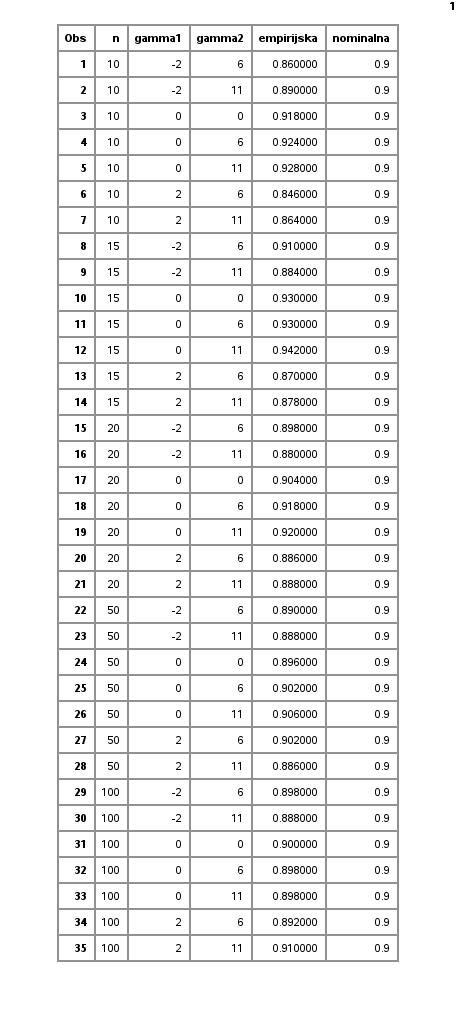
\includegraphics[width=0.5\textwidth]{assets/tablica90.png}
	\caption{Tablica s rezultatima, nominalno 90\%-p.i.}
	\label{tablica90}
\end{figure}


\begin{figure}[h]
	\centering
	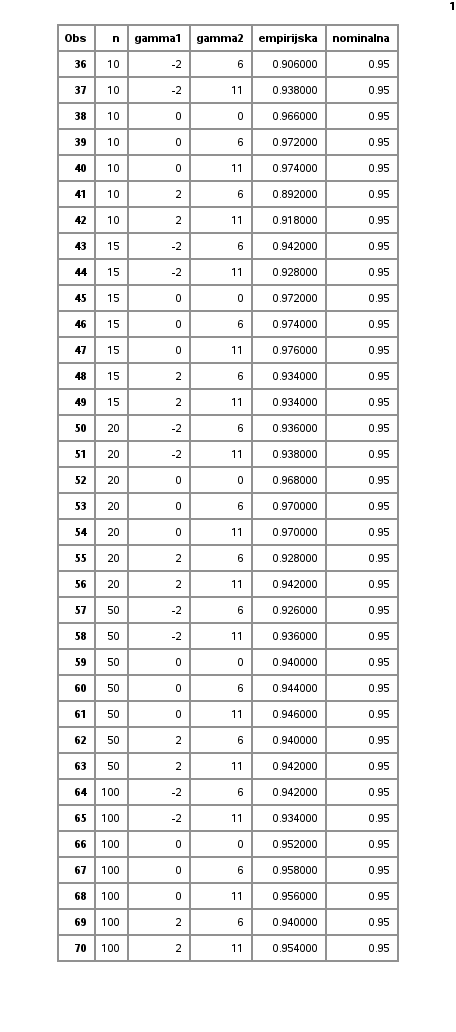
\includegraphics[width=0.5\textwidth]{assets/tablica95.png}
	\caption{Tablica s rezultatima, nominalno 95\%-p.i.}
	\label{tablica95}
\end{figure}


\begin{figure}[h]
	\centering
	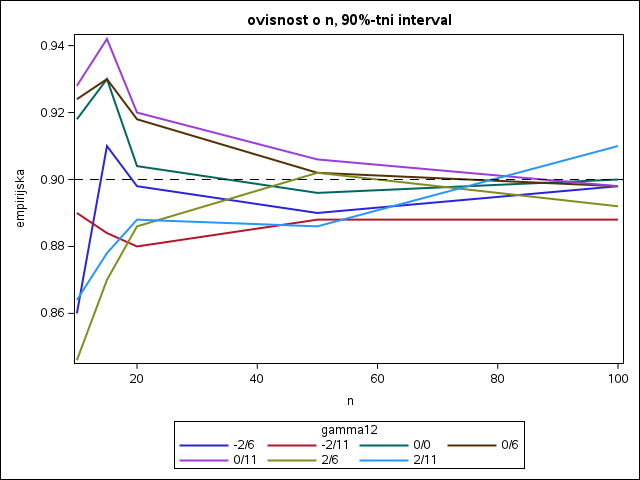
\includegraphics[width=0.5\textwidth]{assets/grafn90.png}
	\caption{Ovisnost vjerojatnosti o \( n \) za fiksne \( \gamma_1, \gamma_2 \), 90\%-p.i.}
	\label{grafn90}
\end{figure}


\begin{figure}[h]
	\centering
	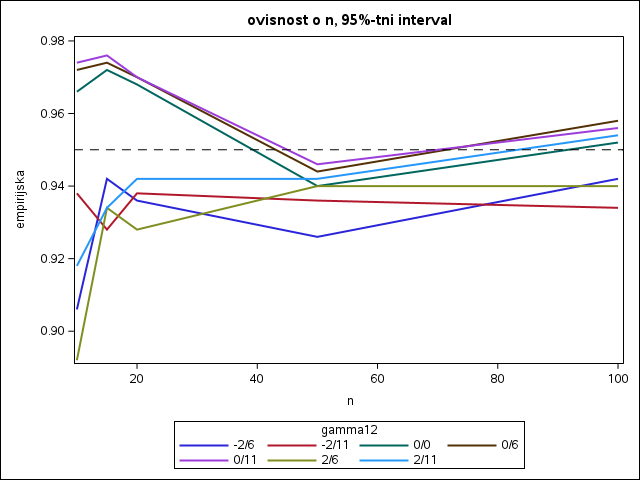
\includegraphics[width=0.5\textwidth]{assets/grafn95.png}
	\caption{Ovisnost vjerojatnosti o \( n \) za fiksne \( \gamma_1, \gamma_2 \), 95\%-p.i.}
	\label{grafn95}
\end{figure}


\begin{figure}[h]
	\centering
	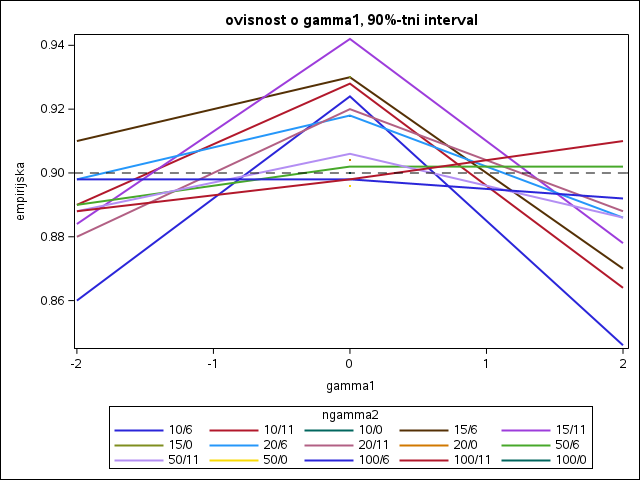
\includegraphics[width=0.5\textwidth]{assets/graf190.png}
	\caption{Ovisnost vjerojatnosti o \( \gamma_1 \) za fiksne \( n, \gamma_2 \), 90\%-p.i.}
	\label{graf190}
\end{figure}

\begin{figure}[h]
	\centering
	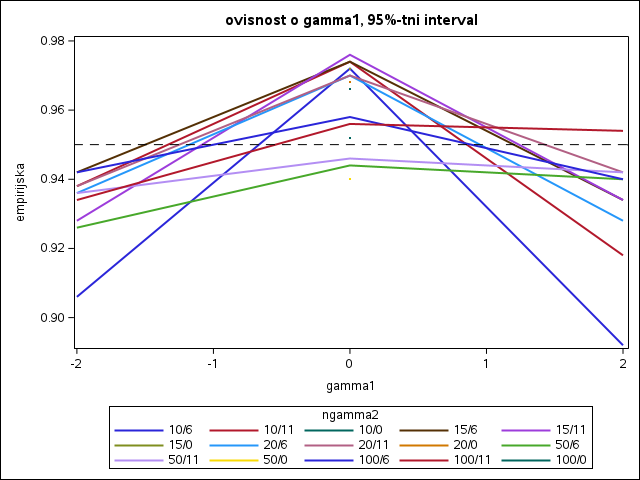
\includegraphics[width=0.5\textwidth]{assets/graf195.png}
	\caption{Ovisnost vjerojatnosti o \( \gamma_1 \) za fiksne \( n, \gamma_2 \), 95\%-p.i.}
	\label{graf195}
\end{figure}

\begin{figure}[h]
	\centering
	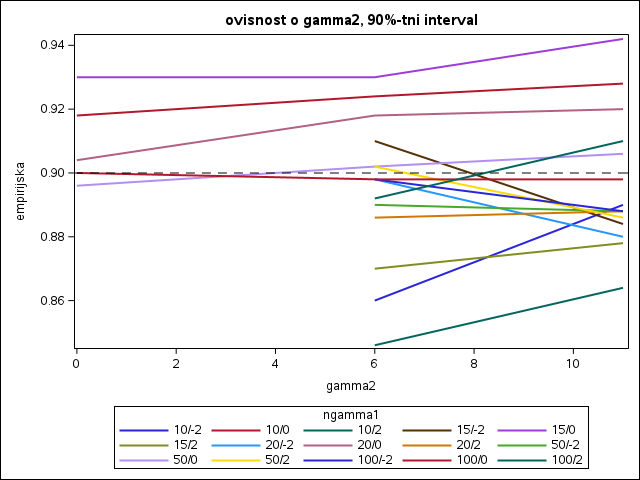
\includegraphics[width=0.5\textwidth]{assets/graf290.png}
	\caption{Ovisnost vjerojatnosti o \( \gamma_2 \) za fiksne \( n, \gamma_1 \), 90\%-p.i.}
	\label{graf290}
\end{figure}

\begin{figure}[h]
	\centering
	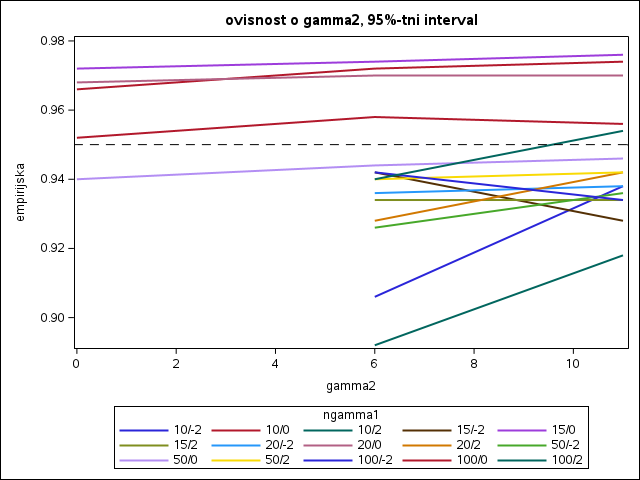
\includegraphics[width=0.5\textwidth]{assets/graf295.png}
	\caption{Ovisnost vjerojatnosti o \( \gamma_2 \) za fiksne \( n, \gamma_1 \), 95\%-p.i.}
	\label{graf295}
\end{figure}

\clearpage

\includepdf{opis.pdf}
\end{document}





